\documentclass[
dbse, % include logo of DBSE work group
  %draft,    % omit title page, listings, and particular chapters selected below using include only
	%german,   % titles for a thesis in German, A4 paper
	%print,    % the printed version does not use colored links
	%final,    % removes all TODOs
]{tex/ttthesis}

% Color Scheme http://colorschemedesigner.com/#3w40I--ALK-K-
% Base Color of the OVGU INF logo, tetraed, -45
\definecolor{blue1}{RGB}{0,105,180} % gray 95
\definecolor{blue2}{RGB}{40,87,121}
\definecolor{blue3}{RGB}{0,57,97}
\definecolor{blue4}{RGB}{76,166,230}
\definecolor{blue5}{RGB}{136,191,230}
\definecolor{orange1}{RGB}{255,144,0} % gray 133
\definecolor{orange2}{RGB}{171,121,56}
\definecolor{orange3}{RGB}{137,78,0}
\definecolor{orange4}{RGB}{255,181,84}
\definecolor{orange5}{RGB}{255,210,151}
\definecolor{green1}{RGB}{11,215,0} % gray 75
\definecolor{green2}{RGB}{52,144,48}
\definecolor{green3}{RGB}{6,116,0}
\definecolor{green4}{RGB}{88,241,80}
\definecolor{green5}{RGB}{148,241,143}
\definecolor{red1}{RGB}{253,0,6} % gray 86
\definecolor{red2}{RGB}{170,56,59}
\definecolor{red3}{RGB}{136,0,3}
\definecolor{red4}{RGB}{254,84,88}
\definecolor{red5}{RGB}{254,151,154}

\definecolor{background}{named}{white}
\definecolor{bgborder}{named}{black}
\definecolor{comment}{named}{red3}

\definecolor{blue}{named}{blue1}
\definecolor{green}{named}{green1}
\definecolor{red}{named}{red1}
\definecolor{orange}{named}{orange1}

\definecolor{pdflinkcolor}{named}{blue3}
\definecolor{pdfcitecolor}{named}{green3}

\usepackage{listings} % source code listings

\lstdefinestyle{java}{
%code formatting
	language=Java,
	tabsize=4,
	breaklines=false,
	basicstyle=\fontfamily{pcr}\footnotesize\selectfont,
	commentstyle=\fontshape{it}\color{darkgray}\selectfont,
	keywordstyle=\fontseries{b}\selectfont,
	stringstyle=\fontfamily{cmr}\selectfont,
%line numbering
	numbers=left,
	numberstyle=\footnotesize,
%frame properties
	captionpos=b,
	frame=single,%trblTRBL
	framesep=3pt,
	xleftmargin=4pt,
	xrightmargin=4pt,
	rulecolor=\color{bgborder},
}

\usepackage{pgfplots}
\usepackage{tikz}
	\usetikzlibrary{arrows,positioning,backgrounds,fit,trees} 
	\usetikzlibrary{fadings,shapes.geometric}
	\usetikzlibrary{decorations,scopes,calc,decorations.pathreplacing}

\ifgerman{
	\pgfplotsset{tick label style={/pgf/number format/1000 sep=.,/pgf/number format/use comma}}
}

% Tortendiagramme
\newcommand{\slice}[4]{
  \pgfmathparse{0.5*#1+0.5*#2}
  \let\midangle\pgfmathresult

  % slice
  \draw[thick,
	%fill=background
	] (0,0) -- (#1:1) arc (#1:#2:1) -- cycle;

  % outer label
  \node[label=\midangle:#4] at (\midangle:1) {};

  % inner label
  \pgfmathparse{min((#2-#1-10)/110*(-0.3),0)}
  \let\temp\pgfmathresult
  \pgfmathparse{max(\temp,-0.5) + 0.8}
  \let\innerpos\pgfmathresult
  \node at (\midangle:\innerpos) {#3};
}
\newcommand{\mypiechart}[2]{
	\begin{tikzpicture}[scale=#1]
		\newcounter{a}
		\newcounter{b}
		\foreach \p/\t in {#2}
			{
				\setcounter{a}{\value{b}}
				\addtocounter{b}{\p}
				\slice{\thea/100*360}
							{\theb/100*360}
							{\p\%}{\t}
			}
	\end{tikzpicture}
}

% surrounding TODOs with this command, gives you the ability to remove all if necessary
\iffinal{
	\newcommand{\todo}[1]{}
	\newcommand{\todots}{}
}{
	\newcommand{\todo}[1]{{\color{comment}\textit{[#1]}}}
	\newcommand{\todots}{\todo{\ldots}}
}
\ifhints{
	\newcommand{\hint}[1]{{\color{hint}\textit{#1}}}
}{
	\newcommand{\hint}[1]{}
}

% propositional formulas
\newcommand{\pand}{\wedge}
\newcommand{\por}{\vee}
\newcommand{\pnot}{\neg}
\newcommand{\pequals}{\Leftrightarrow}
\newcommand{\pimplies}{\Rightarrow}
\newcommand{\pnimplies}{\nRightarrow}
\newcommand{\patmostone}{\mbox{\textit{atmost1}}}
\newcommand{\pchooseone}{\mbox{\textit{choose1}}}

% mathematical definitions and theorems
\newtheorem{definition}{Definition}[chapter]
\newtheorem{theorem}{Theorem}[chapter]
\newtheorem{lemma}{Lemma}[chapter]

% print URLs not in Typewriter Font
\def\UrlFont{\rm}

% empty page without page number, continue on the next right page
\newcommand{\blankpage}{\clearpage{\pagestyle{empty}\cleardoublepage}}

% index stuff
\makeatletter
\def\mydotfill{\leavevmode\xleaders\hb@xt@ .44em{\hss.\hss}\hfill\kern\z@}
\makeatother
\def\bold#1{{\bfseries #1}}
\newbox\dbox \setbox\dbox=\hbox to .4em{\hss.\hss} % dot box for leaders
\newskip\rrskipb \rrskipb=.5em plus3em % ragged right space before break
\newskip\rrskipa \rrskipa=-.17em plus -3em minus.11em % ditto, after
\newskip\rlskipa \rlskipa=0pt plus3em % ragged left space after break
\newskip\rlskipb \rlskipb=.33em plus-3em minus.11em % ragged left before break
\newskip\lskip \lskip=3.3\wd\dbox plus1fil minus.3\wd\dbox % for leaders
\newskip \lskipa \lskipa=-2.67em plus -3em minus.11em %after leaders
\mathchardef\rlpen=1000 \mathchardef\leadpen=600
\def\rrspace{\nobreak\hskip\rrskipb\penalty0\hskip\rrskipa}
\def\rlspace{\penalty\rlpen\hskip\rlskipb\vadjust{}\nobreak\hskip\rlskipa}
\let\indexbreak\rlspace
\def\raggedurl{\penalty10000 \hskip.5em plus15em \penalty0 \hskip-.17em plus-15em minus.11em}
\def\raggeditems{\nobreak\hskip\rrskipb \penalty\leadpen \hskip\rrskipa %
\vadjust{}\nobreak\leaders\copy\dbox\hskip\lskip %
\kern3em \penalty\leadpen \hskip\lskipa %
\vadjust{}\nobreak\hskip\rlskipa}
\renewcommand*\see[2]{\rlspace\emph{\seename}~#1} % from makeidx.sty


%*********************************************************************%
% META                                                                %
%*********************************************************************%
\ifgerman{
  \newcommand{\university}{Otto-von-Guericke-Universität Magdeburg}
  \newcommand{\school}{Fakultät für Informatik}
}{
  \newcommand{\university}{University of Magdeburg}
  \newcommand{\school}{School of Computer Science}
}
\newcommand{\logo}{
\includegraphics[trim=0mm 0mm 50mm 0mm,clip,height=3cm]{INF_SIGN_druck}}
\newcommand{\logodbse}{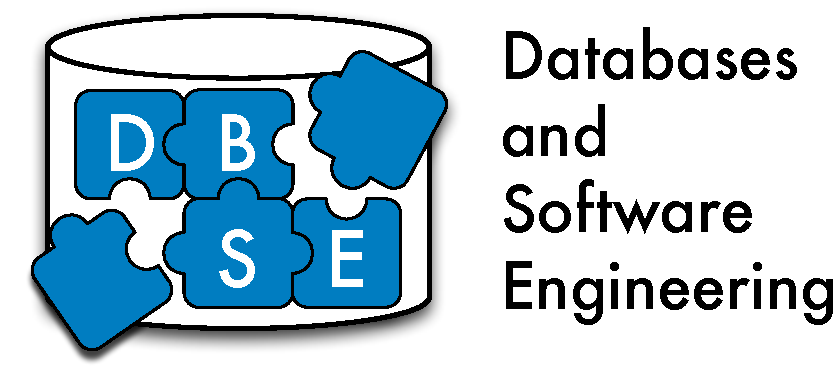
\includegraphics[scale=.45]{DBSE}}

\newcommand{\advisorone}{Prof.\ \todo{Name}}
\newcommand{\departmentone}{\ifgerman{Institut für}{Department of}\todots}

\newcommand{\advisortwo}{}
\newcommand{\departmenttwo}{}

% Thesis kind
\ifgerman{\newcommand{\thesiskind}{Masterarbeit}}{\newcommand{\thesiskind}{Master's Thesis}}
%\ifgerman{\newcommand{\thesiskind}{Bachelorarbeit}}{\newcommand{\thesiskind}{Bachelor Thesis}}
%\newcommand{\thesiskind}{Diplomarbeit} %do not translate
%\ifgerman{\newcommand{\thesiskind}{Doktorarbeit}}{\newcommand{\thesiskind}{Dissertation}}

\ifgerman{
	\newcommand{\theforename}{\todo{Vorname}}
	\newcommand{\thesurname}{\todo{Nachname}}
	\newcommand{\thetitle}{\todo{Titel der Arbeit}}
	\newcommand{\thedate}{\todo{13. Monat}}
}{
	\newcommand{\theforename}{\todo{Forename}}
	\newcommand{\thesurname}{\todo{Surname}}
	\newcommand{\thetitle}{\todo{The Title of the Thesis}}
	\newcommand{\thedate}{\todo{Month 13}}
}
\newcommand{\theyear}{\todo{2013}}

%*********************************************************************%
% SETUP                                                               %
%*********************************************************************%

% meta informations of the document
\hypersetup{
 pdfauthor={\theforename\ \thesurname},
 pdftitle={\thetitle}
}

% open index file
\ifnotdraft{\makeindex}

%*********************************************************************%
% THE DOCUMENT                                                        %
%*********************************************************************%

\begin{document}

% set the path where graphics are located
\graphicspath{{pics/}}

\ifnotdraft{
	\frontmatter
	\pagenumbering{roman}
	\newcommand{\theauthor}{\theforename\ \thesurname}
\newcommand{\theauthorr}{\thesurname,\ \theforename}
\begin{titlepage}
 \thispagestyle{empty}
 \begin{center}
  {\LARGE \university}\\[0.4cm]
  {\Large \school}\\[2.0cm]
  \begin{figure}[h]
   \hbox{}\hfill
    \begin{minipage}[t]{\textwidth}
      \begin{center}
        
\includegraphics[trim=0mm 0mm 50mm 0mm,clip,height=3cm]{INF_SIGN_druck}
      \end{center}
    \end{minipage} 
   \hfill\hbox{}
  \end{figure}\ \\[0.4cm]
  {\huge \thesiskind \\[1.6cm]}
  {\Large\bf \thetitle \\[1.6cm]}
  {\small Author:}\\[0.4cm]
  {\large \theauthor}\\[0.8cm]
  {\large \thedate, \theyear}\\[0.8cm]
  {\small Advisors:}\\[0.4cm] 
  {\large
\advisorone
  }\\[0.2cm]
  {\small
\departmentone
  }\\[0.8cm]
  {\large
\advisortwo\ 
  }\\[0.2cm]
  {\small
\departmenttwo\ 
  }
 \end{center}
\end{titlepage}

%%%%%%%%%%%%%%%%%%%%%%%%%%%%%%%%%%%%%%%%%%%%%%%%%%%%%%%%%%%%%%%%%%%%%%%%%%%%
%%% Titelr�ckseite: Bibliographische Angaben
%%%%%%%%%%%%%%%%%%%%%%%%%%%%%%%%%%%%%%%%%%%%%%%%%%%%%%%%%%%%%%%%%%%%%%%%%%%%

\thispagestyle{empty}
\vspace*{\fill}
\begin{minipage}{15.0cm}
\textbf{\theauthorr:}\\
\emph{\thetitle\\}
\thesiskind, \university, \theyear.
\end{minipage}
\newpage


	\ifgerman{\chapter*{Inhaltsangabe}}{\chapter*{Abstract}}

\todots

	\blankpage

	%\chapter*{Acknowledgements}
	%\ldots
	%\blankpage
}

%*********************************************************************%
% ACRONYMS                                                            %
%*********************************************************************%

% HOWTO: \gls{IDE} for singular or \glspl{IDE} for plural with 's
\makeglossaries
\newacronym{IDE}{IDE}{Integrated Development Environment}
%\glsaddall % use only if you have acronyms that occur only in graphics

%*********************************************************************%
% LISTINGS                                                            %
%*********************************************************************%

\ifnotdraft{
	{\parskip 0pt\tableofcontents} % toc bitte einzeilig
	\blankpage

	\ifgerman{
		\listoffigures
		\addcontentsline{toc}{chapter}{Abbildungsverzeichnis}

		\listoftables
		\addcontentsline{toc}{chapter}{Tabellenverzeichnis}

		\renewcommand{\lstlistlistingname}{Quelltextverzeichnis}
		\lstlistoflistings
		\addcontentsline{toc}{chapter}{Quelltextverzeichnis}

		\renewcommand*{\firstacronymfont}[1]{\emph{#1}}
		\printglossary[type=acronym,title=List of Acronyms,toctitle=Abkürzungsverzeichnis]
	}{
		\listoffigures
		\addcontentsline{toc}{chapter}{List of Figures}

		\listoftables
		\addcontentsline{toc}{chapter}{List of Tables}

		\renewcommand{\lstlistlistingname}{List of Code Listings}
		\lstlistoflistings
		\addcontentsline{toc}{chapter}{List of Code Listings}

		\renewcommand*{\firstacronymfont}[1]{\emph{#1}}
		\printglossary[type=acronym,title=List of Acronyms,toctitle=List of Acronyms]
	}
}

%*********************************************************************%
% CHAPTERS                                                            %
%*********************************************************************%

\mainmatter
\pagenumbering{arabic}

\ifgerman{\chapter{Einführung}}{\chapter{Introduction}}

%- Hintergrund
%- Motivation
%- Ziele
%- Aufgaben
%- Allgemeine Beschreibung des Projektes
%- Worum geht es in dieser Arbeit?
%- Wer hat die Arbeit veranlasst und wozu?
%- Wer soll von den Ergebnissen profitieren?
%- Welches Problem soll gelöst werden? Warum?
%- Unter welchen Umständen braucht man eine Verbesserung?
%- Was ist der Stand der Technik?
%- Welche noch offenen Probleme gibt es?
%- Worin unterscheidet sich mein Ansatz von den bisherigen?
%- Welche Ziele hat die Arbeit?
%- Wie will ich diese Ziele erreichen?
%- Was habe ich im Einzelnen vor?

\hint{}

\hint{\ldots\ to be continued \ldots}

\todots

\ifgerman{\paragraph{Zielstellung der Arbeit}}{\paragraph{Goal of this Thesis}}

\todots

\ifgerman{\paragraph{Gliederung der Arbeit}}{\paragraph{Structure of the Thesis}}

\todots

\ifgerman{\chapter{Grundlagen}}{\chapter{Background}}
\label{background}
%- Allgemeine Wissensgrundlagen des Fachgebiets
%- Spezielle Grundlagen, die f�r das Verst�ndnis erforderlich sind
%- Rahmenbedingungen f�r die Arbeit
%- Ausf�hrungen zum Stand des Wissens / der Technik
%Als Leitprinzip gilt: Nur Informationen erw�hnen, die
%- sp�ter ben�tigt werden,
%- notwendig sind, um die Arbeit oder ihre Motivation zu verstehen
%Das hei�t insbesondere,
%- keine Inhalte aus Lehrb�chern, au�er
%- diese werden ben�tigt, um Problemstellung oder L�sungsweg zu definieren.

\todots
\chapter{Example Chapter}
\label{ch:example}
%In diesem Kapitel beschreiben Sie Ihren eigenen Beitrag
%- Es muss klar sein, worin die eigentliche Innovation besteht#

This chapter gives you some examples how to include graphics, create tables, or include code listings. But first, we start with a short description how you can efficiently cite in \LaTeX. The following footnote shows you how to reference URLs and where this document is available online.\footnote{\url{http://www.ovgu.de/tthuem}}

%\section{Acronyms}
%
%This template makes advantage of the glossaries package to support acronyms. The first occurence of an acronym is replaced by its definition (e.g., \gls{IDE}). All other occurences are replaced by the acronym (\gls{IDE}). The glossaries package also supports plural---\glspl{IDE}.
%
%\glsreset{IDE}
%Sometimes you want to make sure, that the long version is used, even if \gls{IDE} was inserted before.

\section{Citation}

There are several types of literature. The most citations are workshop and conference papers. Please use the inproceedings-tag for those citations (e.g., \cite{KAK:GPCE09}). You should have short-hands for workshop and conference names to be sure the naming is consistent and uniform (see our BibTeX files how to do that).

Slightly different are articles published in journals (e.g., \cite{KG:SME06}). Make sure you that the volume and number-tags are present and that no inproceeding is tagged as article or vice versa.

You might want to take a look at the example BibTeX file to find out how to cite books~\cite{CE:BOOK00}, technical reports~\cite{KCHNP:TR90}, websites~\cite{Coq:website}, PhD theses, or master theses~\cite{B:PHD03,R:MT09}.

\section{Formulas}

There are different types of mathematical environments to set formulas. The equation $E=m\cdot c^2$ is an inline formula. But you can also have formulas at a separate line (see \vref{eq:ex}).

	\begin{equation}\label{eq:ex}
			P=\bigl(\mathcal{A}\pimplies(\mathcal{B}\pequals\mathcal{C})\pand(\mathcal{B}\pequals\mathcal{D})\bigr)\pand(\mathcal{B}\pimplies\mathcal{A})\pand(\mathcal{C}\pimplies\mathcal{A})\pand(\mathcal{D}\pimplies\mathcal{A})
	\end{equation}

If you need multiple lines that are aligned to each other, you might want to use the following code.

	\newcommand{\fG}{\mbox{GraphLibrary}}
	\newcommand{\fE}{\mbox{Edges}}
	\newcommand{\fA}{\mbox{Algorithms}}
	\newcommand{\fD}{\mbox{Directed}}
	\newcommand{\fU}{\mbox{Undirected}}
	\newcommand{\fN}{\mbox{Number}}
	\newcommand{\fC}{\mbox{Cycle}}
	\begin{eqnarray*}
	&& \fG\\
	&\pand& (\fG \pimplies \fE) \pand (\fE \por \fA \pimplies \fG)\\
	&\pand& (\fE \pequals \fD \por \fU) \pand (\pnot \fD \por \pnot \fU)\\
	&\pand& (\fA \pequals \fN \por \fC)\\
	&\pand& (\fC \pimplies \fD).\\
	\end{eqnarray*}

\section{Graphics}

In \vref{fig:ex}, we give a small example how to insert and reference a figure.

\begin{figure}[htbp]
	\centering
		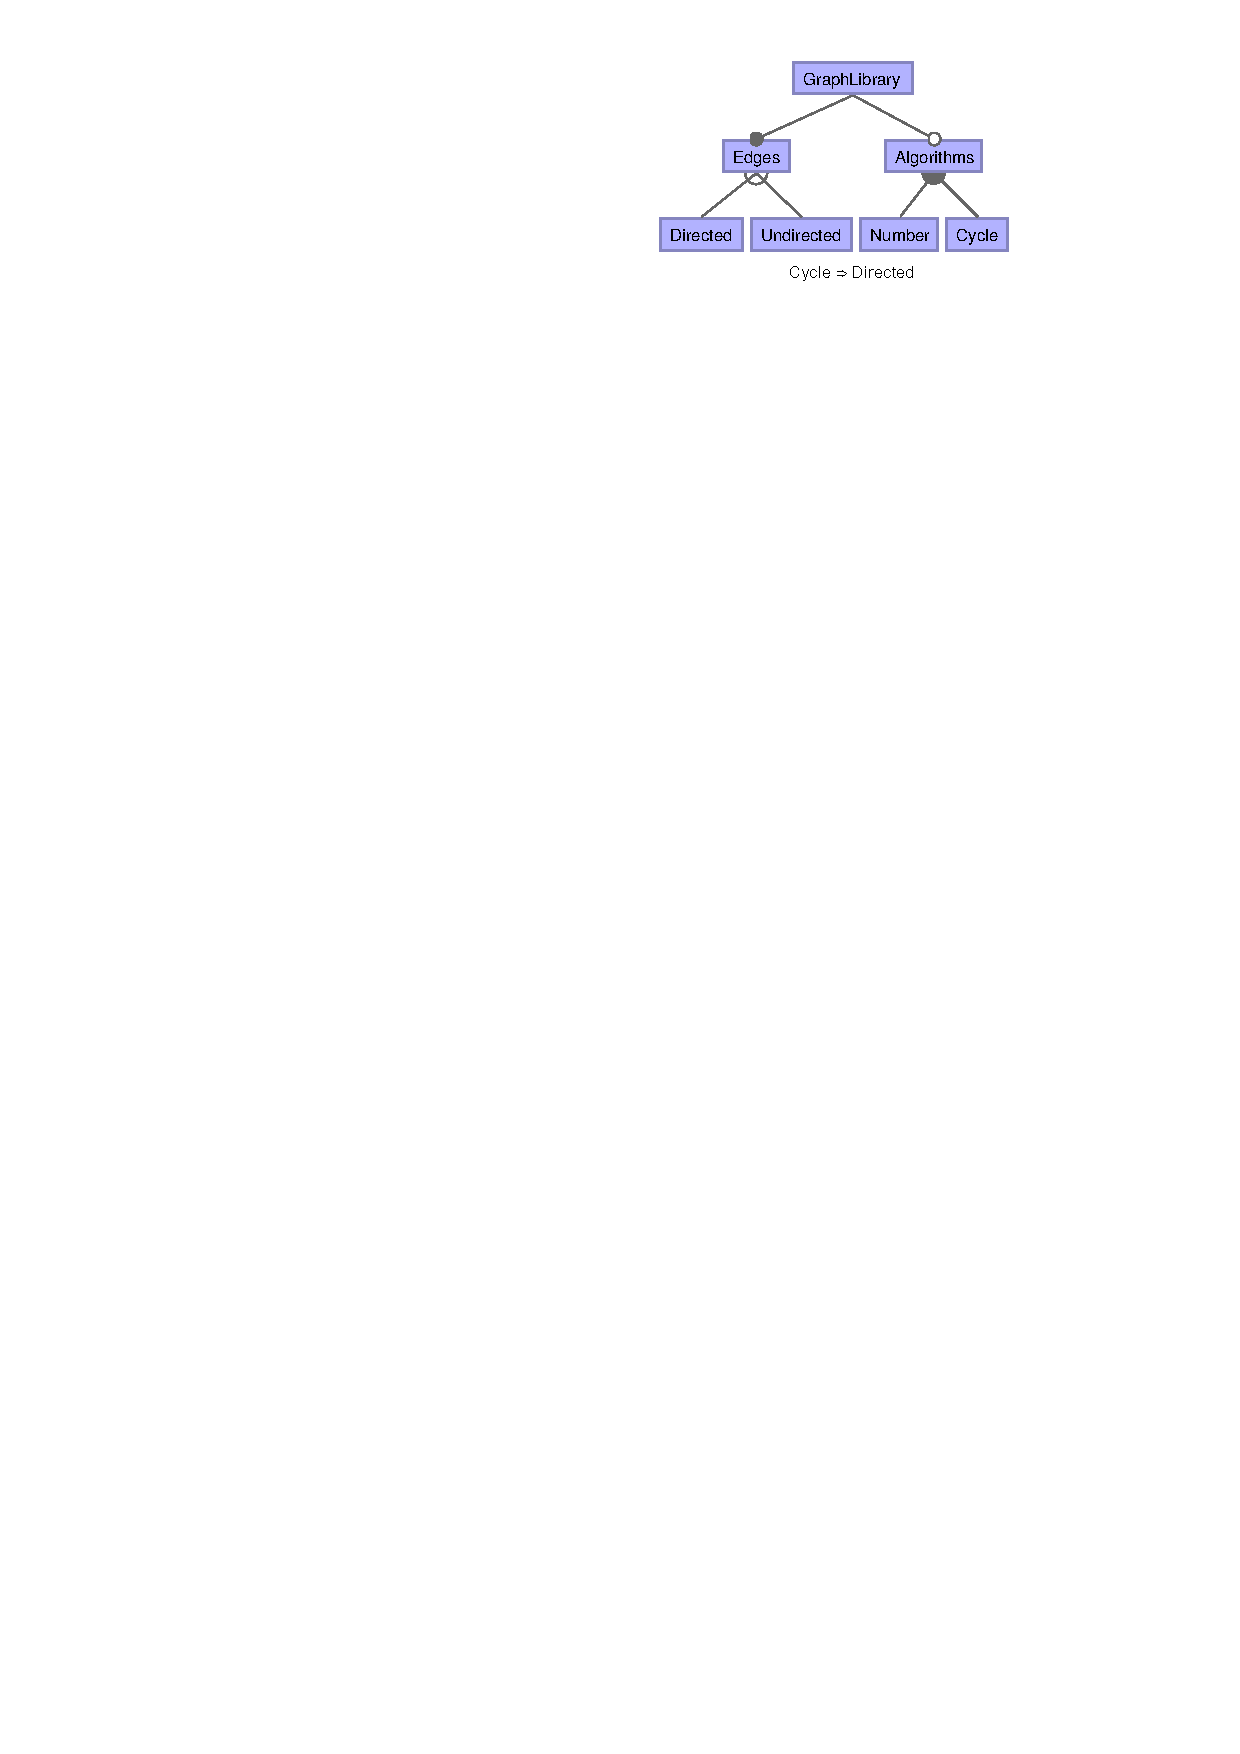
\includegraphics[scale=1.25]{example}
	\caption{A feature model representing a graph product line}
	\label{fig:ex}
\end{figure}

\section{Tables}

\vref{tab:ex} shows the result of a simple tabular environment.

\begin{table}[htbp]
	\centering
		\begin{tabular}{cc}\toprule
			Group Type & Propositional Formula\\\midrule
			And & $(P \pimplies C_{k_1} \wedge\ldots\wedge C_{k_m}) \pand (C_1\vee\ldots\vee C_n \pimplies P)$\\\addlinespace
			Or & $P \pequals C_1\vee\ldots\vee C_n$\\\addlinespace
			Alternative & $(P \pequals C_1\vee\ldots\vee C_n) \pand \mbox{atmost}1(C_1,\ldots,C_n)$\\
			\bottomrule
		\end{tabular}
	\caption{Mapping a feature model to a propositional formula}
	\label{tab:ex}
\end{table}

\section{Code Listings}

In \vref{lst:ex}, we give an example of a source code listing. 

\begin{lstlisting}[style=Java,float=htb,caption={Java source code},label={lst:ex}]
class A extends Object {
	A() { super(); }
}
class B extends Object {
	B() { super(); }
}
class Pair extends Object {
	Object fst;
	Object snd;
	Pair(Object fst, Object snd) {
		super(); this.fst=fst; this.snd=snd;
	}
	Pair setfst(Object newfst) {
		return new Pair(newfst, this.snd);
	}
}
\end{lstlisting}

\chapter{Evaluation}
\label{evaluation}
%Die Beurteilung ist einer der wichtigsten Abschnitte der Arbeit
%- Sie enth�lt die Quintessenz des gesamten Projektes
%Viele lesen nur die Einf�hrung und die Beurteilung an
%- Hier muss also alles Wichtige drin stehen!
%Hier beweisen Sie dass Sie �
%- die Aufgabe und deren Bedeutung verstanden haben
%- die Ergebnisse richtig zu interpretieren verm�gen
%- wissen, worauf es bei diese Arbeit ankam

\todots
\ifgerman{\chapter{Verwandte Arbeiten}}{\chapter{Related Work}}
\label{relatedwork}

\todots

\ifgerman{\chapter{Zusammenfassung und zukünftige Arbeiten}}{\chapter{Conclusion and Future Work}}
\label{ch:conclusion}

\todots
\chapter{Future Work}
\label{futurework}

\todots

%*********************************************************************%
% APPENDIX                                                            %
%*********************************************************************%

\appendix
\ifgerman{\chapter{Anhang}}{\chapter{Appendix}}
\label{appedixa}

\todots

%*********************************************************************%
% LITERATURE                                                          %
%*********************************************************************%

\cleardoublepage
\phantomsection
\addcontentsline{toc}{chapter}{\bibname} % 
\bibliographystyle{alpha} % plain gerplain abbrvnat unsrtnat alphag alpha
% in a thesis you have space... use full names
\bibliography{literature/IEEEfull,literature/MYfull,literature/literature}
% in a paper, space is limited. use abreviations
%\bibliography{../literature/IEEEabrv,../literature/MYabrv,../literature/literature}

%*********************************************************************%
% ERKLÄRUNG                                                           %
%*********************************************************************%

\ifnotdraft{
	\cleardoublepage
	\phantomsection
	\printindex
	\thispagestyle{empty}
\vspace*{38\baselineskip}
\hbox to \textwidth{\hrulefill}
\par
Hiermit erkl�re ich, dass ich die vorliegende Arbeit selbst�ndig verfasst und
keine anderen als die angegebenen Quellen und Hilfsmittel verwendet habe.

Magdeburg, den \todots

%%%%%%%%%%%%%%%%%%%%%%%%%%%%%%%%%%%%%%%%%%%%%%%%%%%%%%%%%%%%%%%%%%%%%%%%
%% Hinweis:
%%
%% Diese Erkl�rung wird von der Pr�fungsordnung f�r Diplomarbeiten 
%% verlangt und ist zu unterschreiben. F�r Studienarbeiten ist diese
%% Erkl�rung nicht zwingend notwendig, schadet aber auch nicht.
%%%%%%%%%%%%%%%%%%%%%%%%%%%%%%%%%%%%%%%%%%%%%%%%%%%%%%%%%%%%%%%%%%%%%%%%
\clearpage

}

\end{document}
